\section{Numerical Experiments}
We provide numerical evidence supporting our conclusions.


\subsection{Simulating Lemma \ref{lemma:free}}\label{subsec:lemma sims}
Lemma \ref{lemma:free} is used to construct D-optimal designs as a
part of the proof of Theorem \ref{thm:char}. We implement the
construction in Lemma \ref{lemma:free} (see module \texttt{zeros.py}
in the accompanying
\href{https://github.com/yairdaon/OED}{repository}). We iterate over
the number of measurements $m \in \{4,\dots, 15\}$, and for every $m$
we then iterate over $k:=\rank \obs^*\obs \in \{2,\dots, m-1\}$. For
each pair $m,k$ we run $N=50000$ simulations according to the
following steps:
\begin{enumerate}
\item Generate random diagonal $D\in \mathbb{R}^{k\times k}$ and
  normalize it so that $\ttr D = m$.
\item Conjugate $D$ by a random orthogonal matrix to form a positive
  semi-definite $M := UDU^t \in \mathbb{R}^{k\times k}$.
\item Apply the construction of Lemma \ref{lemma:free} to calculate
  $A$ such that $AA^t = M$, where $A$ has unit norm columns.
\item We call $A$ "clustered" if $A$ has two or more identical columns
  (up to some numerical precision threshold).
\end{enumerate}
We then calculate the fraction of clustered designs of the $N=5000$
simulations we ran, for each pair $m,k$. Full results in the
\texttt{simulations.csv} file within the accompanying
\href{https://github.com/yairdaon/OED}{repository}), below we give a
brief description of the results.

Clusteriztion occured at high rates ($>95\%$) whenever $m-k > 1$; see
Fig.~\ref{fig:sim AAt}. Hence, in these simulations, clusterization is
a generic property. However, when $m-k \leq 2$, clusterization does
not occur. We do not why and further investigation into this
phenomenon is out of scope for the current study.

\begin{figure}
    \centering
    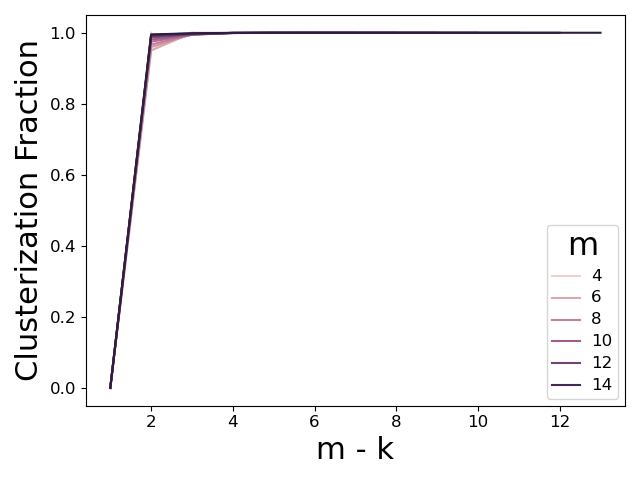
\includegraphics[height=0.5\textwidth]{simulations.png}
    \caption{Fraction of clustered $A$ for $AA^t = M$ and $M$
      generated randomly (see text and repository for details on
      generating $M$). It is evident that when $m-k >3$ clusterization
      is ubiquitous, whereas for lower $m-k$ clusterization does not
      occur.}
  \label{fig:sim AAt}
\end{figure}


\subsection{Correlated errors}\label{subsec:corr errors sims}
In order to verify the results of Section \ref{section:non vanishing},
we run simulations of the inverse problem of the 1D heat equation
\ref{subsec:1d heat} with nonvanishing model error. We take a model
correlation of \(\modcov = \prcov^2 \). Indeed, adding model
correlation pushes measurements apart as can be seen in
Fig.~\ref{fig:corr errors}. Code generating the image below can be
located at module \texttt{clusterization.py} in the accompanying
\href{https://github.com/yairdaon/OED}{repository}).

\begin{figure}
    \centering
    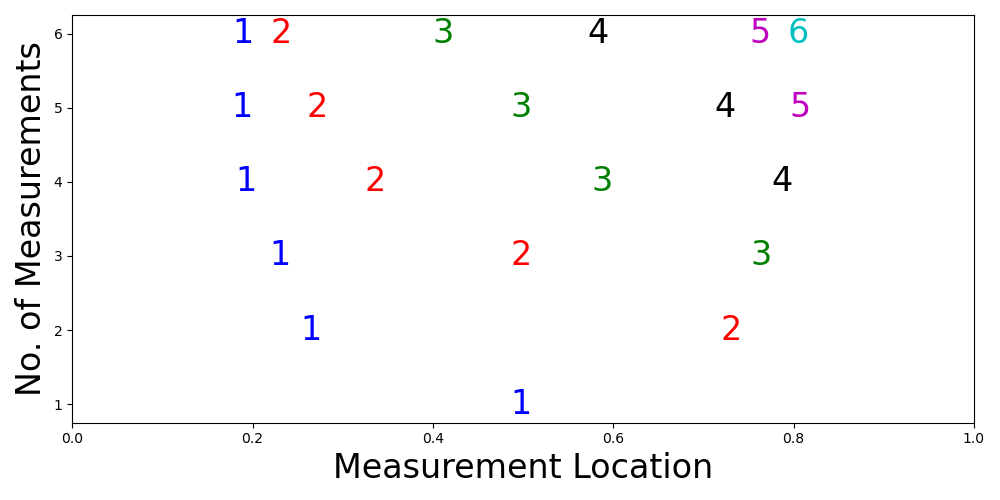
\includegraphics[height=0.5\textwidth]{dst_modelError4.png}
    \caption{Model correlation mitigates clusterization. We add a
      model correlation term to the error terms in the 1D heat
      equation inverse problem. Lo and behold, measurements are not
      close anymore and are pushed away thanks to the model error
      term.}
  \label{fig:corr errors}
\end{figure}
